\def\nr{11. Aufgabenblatt}
\def\kopf{\\\hfill\normalsize\mdseries}
\documentclass[11pt,a4paper,fleqn]{scrartcl}
\usepackage{eurosym}
\usepackage{adjustbox,csquotes}
%\usepackage{a4kopka}
\usepackage{amsmath,amssymb,amsthm,amsfonts}
\usepackage[utf8]{inputenc}
\usepackage{algorithmic,algorithm}
\usepackage{graphics,graphicx}
\usepackage{pgfplots,tikz}
\usepackage{enumerate}
\usepackage[ngerman]{babel}
% \usepackage[software]{mymacros}
%\usepackage{matrix}
\usepackage{hyperref}
% \usepackage{caption}
\usepackage{caption, subcaption}

\floatname{algorithm}{Algorithmus}
\renewcommand{\algorithmicrequire}{\textbf{Input:}}
\renewcommand{\algorithmicensure}{\textbf{Output:}}

%\usepackage{enumitem} 
%\textheight25cm
\textheight23cm
\topmargin-15mm
\oddsidemargin-5mm    %  -10mm
\textwidth17cm    %   18.8cm
\footskip0pt
\thispagestyle{empty}
\parindent0mm
\parskip0ex
\parskip0ex

\makeatletter
\DeclareOldFontCommand{\rm}{\normalfont\rmfamily}{\mathrm}
\DeclareOldFontCommand{\sf}{\normalfont\sffamily}{\mathsf}
\DeclareOldFontCommand{\tt}{\normalfont\ttfamily}{\mathtt}
\DeclareOldFontCommand{\bf}{\normalfont\bfseries}{\mathbf}
\DeclareOldFontCommand{\it}{\normalfont\itshape}{\mathit}
\DeclareOldFontCommand{\sl}{\normalfont\slshape}{\@nomath\sl}
\DeclareOldFontCommand{\sc}{\normalfont\scshape}{\@nomath\sc}
\makeatother

% \newcommand{\cg}[1]{{\color{blue} #1}}
% \newcommand{\cb}[1]{{\color{green} #1}}
% \newcommand{\cred}[1]{{\color{red} #1}}
% \newcommand{\cc}[1]{{\color{cyan} #1}}
% \newcommand{\cm}[1]{{\color{magenta} #1}}

\newcommand{\Aufgabe}[2][]{\par\bigskip{\sf\bfseries Aufgabe #2#1:}}
%\hspace{3em}{\small(#2 point\ifthenelse{#2>1}{s}{})}}\par\smallskip}
%\newcommand\aufgabe[2][~]{\par\bigskip{\sf\bfseries Aufgabe #1
%    \hspace{3em} \ifthenelse{\equal{#2}{~}}{}{(#2)}}\par\smallskip}
\usepackage{mymacros}

\begin{document}
{\sf Universit\"at Hamburg \hfill Wintersemester 2020/21 \\ Fachbereich Mathematik \\ Dr. Matthias Voigt}
\begin{center}
\ifthenelse{\equal{\nr}{no}}{\Large\sf\bfseries \kopf}{\Large\sf\bfseries Optimierung f\"ur Studierende der Informatik -- \nr.~\kopf}
\end{center}

\renewcommand{\tilde}{\widetilde}
\renewcommand{\hat}{\widehat}
\newcommand{\ri}{\mathrm{i}}
\renewcommand{\H}{\mathsf{H}}
\newcommand{\T}{\mathsf{T}}


\subsection*{Präsenzaufgaben am 01./02.02.2021}

\Aufgabe[ (gewichtete Hitting-Sets)]{P1}
Gegeben sei eine Menge $S = \bigl\{ s_1,\ldots,s_n \bigr\}$ und eine Kollektion $T_1,\ldots,T_m$ von $k$-elementigen Teilmengen von $S$. Außerdem besitze jedes Element $s_i$ ein Gewicht $w_i \geq 0$ mit $w_i \in \mathbb{Q}$ ($i=1,\ldots,n$).

Zur Erinnerung: Eine Teilmenge $H \subseteq S$ wird ein \textit{Hitting-Set} genannt, falls $H \cap T_i \neq \emptyset$ für alle $i=1,\ldots,m$ gilt. Gesucht ist ein Hitting-Set $H$, dessen Gewicht so klein wie möglich ist. Anders gesagt: Die Summe
\[
\sum\limits_{s_i \in H}{w_i}
\]
soll so klein wie möglich sein. Wir wollen das beschriebene Problem als {\glqq}gewichtetes $k$-Hitting-Set-Problem{\glqq} bezeichnen.

\begin{enumerate}[a)]
% Aufgabe P-1a
\item Formulieren Sie dieses Problem als ein ganzzahliges Programmierungsproblem, dass Sie (ILP) nennen.
% Aufgabe P-1b
\item Wie lautet die LP-Relaxation (LP) dieses Problems?
\end{enumerate}

\Aufgabe[ (Dijkstra-Algorithmus)]{P2}
Der Graph $G = (V,E)$ mit Längenfunktion $\ell$ sei durch die folgende Zeichnung gegeben:

\begin{center}
 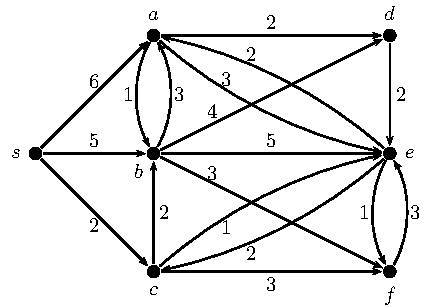
\includegraphics[width = 0.6\linewidth]{fig11_1.pdf}
\end{center}



\begin{enumerate}[a)]
% Aufgabe P-2a
\item Verwenden Sie den modifizierten Algorithmus von Dijkstra, um für alle $v \in V$ die Länge $d(v)$ eines kürzesten $s,v$-Pfades zu berechnen. Legen Sie eine Tabelle wie auf Folie 32 aus Vorlesung 11 an, d.h., notieren Sie auch immer einen \enquote{Vorgängerknoten}.

% Aufgabe P-2b
\item Bestimmen Sie einen kürzeste-Pfade-Baum anhand der Einträge in der letzten Zeile Ihrer Tabelle.
\end{enumerate}


\subsection*{Hausaufgaben bis zum 10.02.2021 (12:00 Uhr)}
\emph{Bitte reichen Sie Ihre Hausaufgaben in festen Zweier- oder Dreiergruppen bei Moodle ein. Bitte laden Sie ausschließlich \textbf{PDF-Dokumente} hoch, andernfalls können Ihre Hausaufgaben nicht korrigiert werden.}

\Aufgabe[ (Dijkstra-Algorithmus, 4 Punkte)]{H1}
Der Graph $G=(V,E)$ mit Längenfunktion $\ell$ sei durch die folgende Zeichnung gegeben:

\begin{center}
 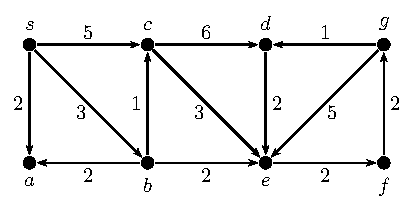
\includegraphics[width = 0.54\linewidth]{fig11_2.pdf}
\end{center}

Verwenden Sie den modifizierten Algorithmus von Dijkstra (Vorlesung 11, Folie 24) um für alle $v \in V$ die Länge $d(v)$ eines kürzesten $s,v$-Pfades zu berechnen. Legen Sie eine Tabelle an, an der man zusätzlich kürzeste $s,v$-Pfade ablesen kann. Bestimmen Sie auch einen kürzeste-Pfade-Baum. 

\Aufgabe[ (minimale aufspannende Bäume, 6 Punkte)]{H2}
Für den folgenden Graphen bestimme man einen minimalen aufspannenden Baum auf drei Arten:
\begin{enumerate}[a)]
\item mit dem Algorithmus von Kruskal;
\item mit dem Algorithmus von Prim (mit Startknoten $a$);
\item mit dem Reverse-Delete-Algorithmus.
\end{enumerate}

Geben Sie jeweils die Kanten in der Reihenfolge an, in der sie hinzugefügt bzw. weggelassen wurden. (Kommen mehrere Kanten infrage, so wähle man willkürlich eine aus.)

\begin{center}
 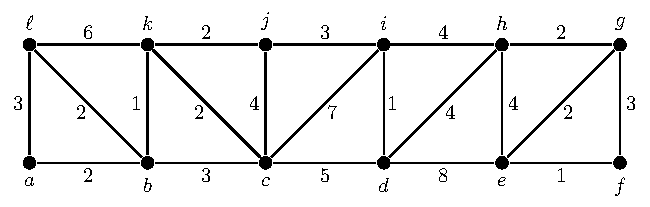
\includegraphics[width = 0.9\linewidth]{fig11_3.pdf}
\end{center}

\end{document}
